% This section describes the design of the memory system model. How host target
% decoupling is achieved. What configurations are available.

Our memory timing-model \textit{generator} describes a space of
\textit{instances}, each of which may be used to model a restricted set of
memory systems. As input, the generator accepts a configuration that specifies
the static parameters of the instance,  such as width of the interfaces it
binds to, the number of outstanding requests it must support, and the type of
memory system the instance will model (a \emph{timing-model class}). As output,
the generator produces an instance module and local memory map of all registers
it will exposes to the simulation interconnect. These registers control timing
parameters can be overwritten to reconfigure the instance without needing to
regenerate it.

Instances operate by using the FPGA host's off-chip memory system as a backing
store: target requests carried through simulation tokens are snooped by the
\emph{ingress unit} and re-issued to the host-memory system. Responses from the
host-memory system are subsequently buffered by the \emph{egress unit}. In
parallel, a host-decoupled \emph{timing-model} explicitly consumes input tokens
and generates output tokens. When the timing-model wishes to release a token
with a valid target response, it fetches the matching host response from the
egress unit. If no host response is present, the timing-model does not produce
a token. This preserves simulation timing regardless of host-memory system
timing.

A block diagram of an instance is shown in figure~\ref{fig:timing_model}.

\begin{figure}
	\centering
	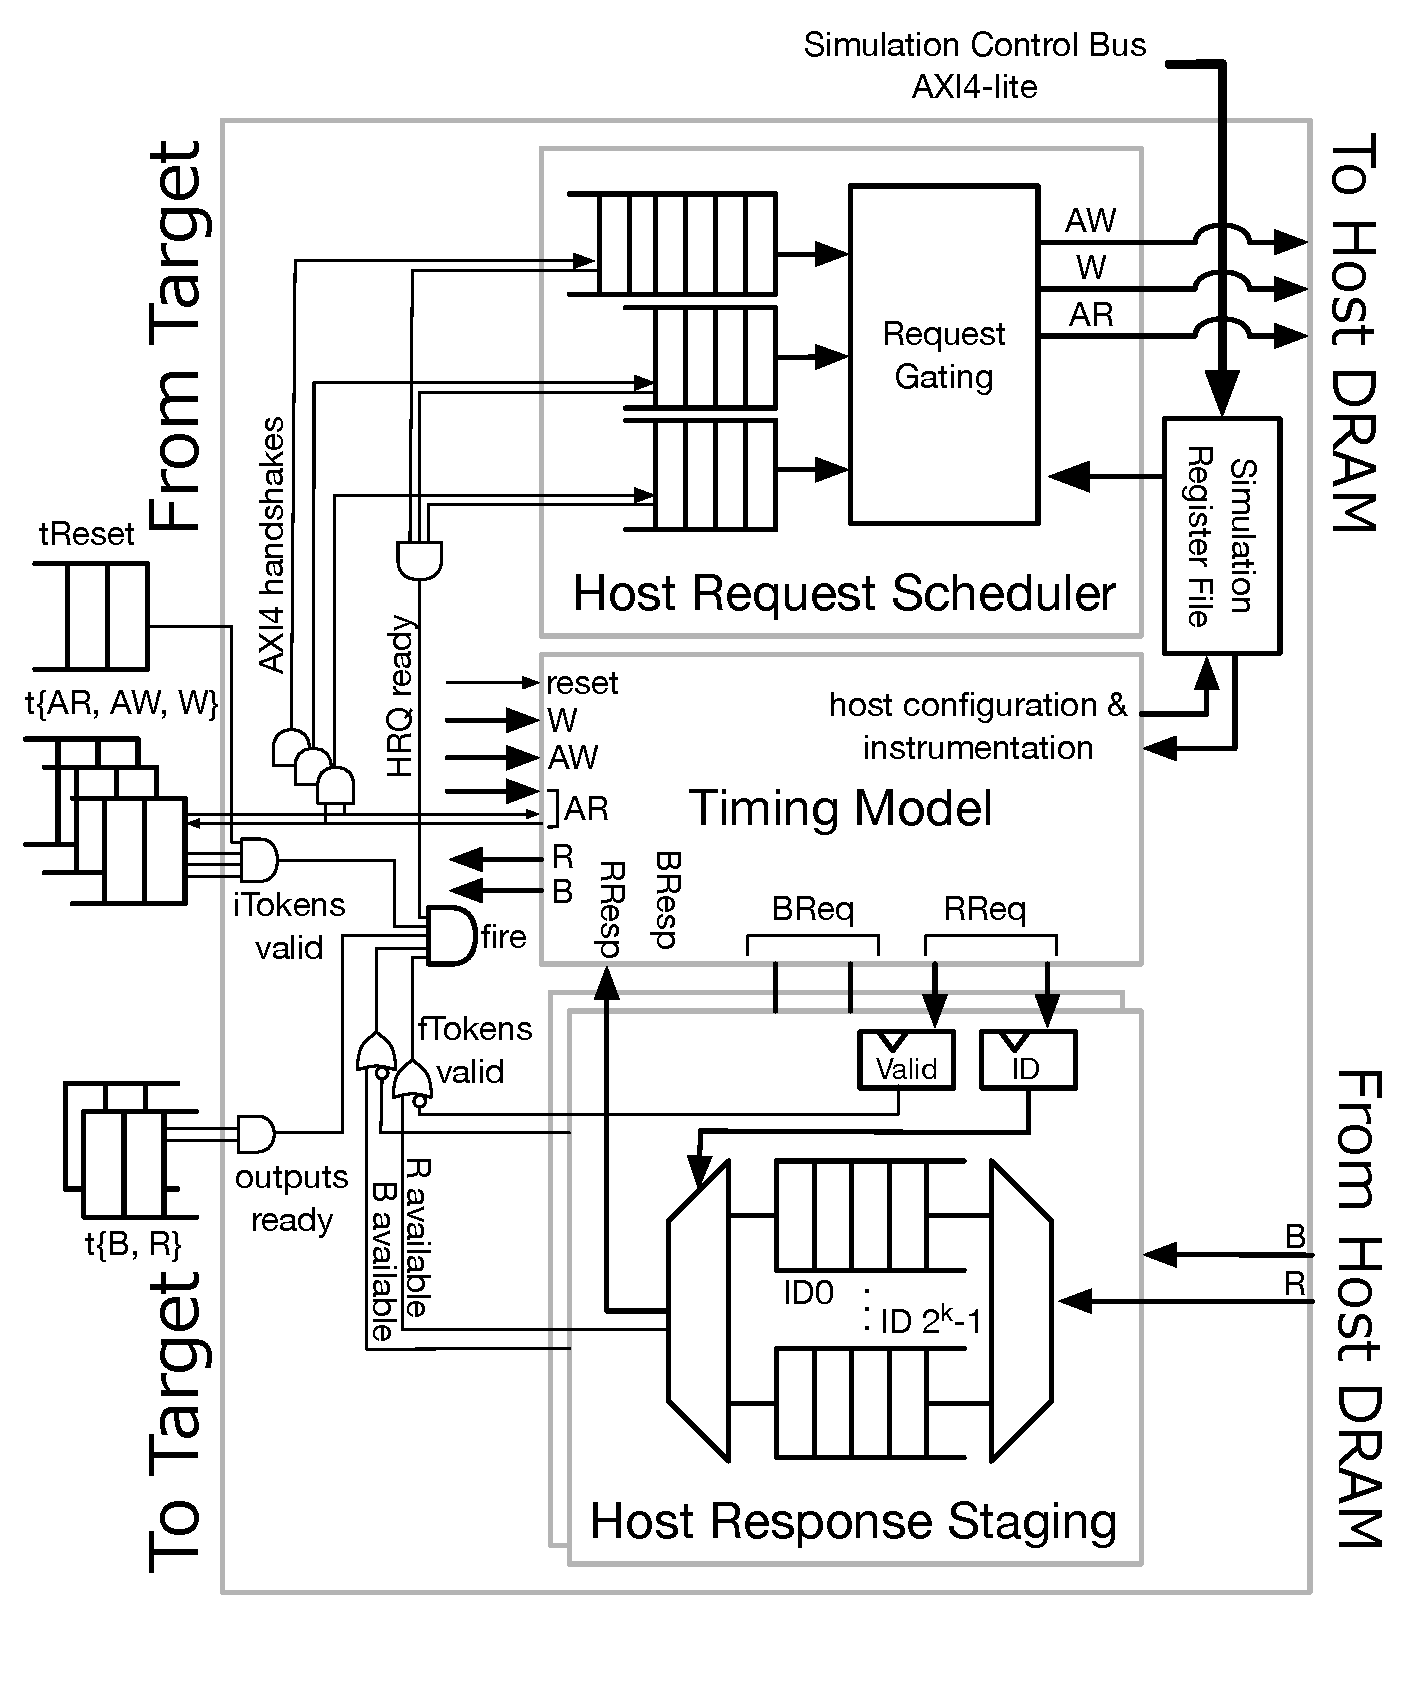
\includegraphics[width=\columnwidth]{figures/memory-model-block-diagram.pdf}
	\caption{Top-level diagram of memory system model with latency-bandwidth pipe timing-model}
	\label{fig:timing_model}
\end{figure}

\section{Interfaces}\label{sec:interfaces}

All instances have three interfaces.

\begin{enumerate}
    \item \textbf{Target-side:} Host-decoupled AXI4 slave
        interface and synchronous reset. AXI4 consists of five ready-valid
        channels; three request channels driven by the master, and two
        response channels driven by the slave.  An input token consists of
        the valids and payloads for each request channel, the readies for
        each response channel, and the synchronous reset.  An output token
        is the complement; the valids and payloads for each response
        channel, and the readies for each request channel.  While tokens
        may be carried to and from the instance on separate timing channels
        (for each AXI4 channel and reset), simulation mapping ensures
        these are fused into a single input token, and fractured into
        multiple output tokens accordingly.

    \item \textbf{Host-side:} AXI4 master. This interface is used by the
        instance to make requests of the host-memory system. It operates
        independently of target-time.

    \item \textbf{Configuration-side:} AXI4-lite slave. This interface exposes both
        memory-mapped configuration registers and instrumentation to the
        simulation interconnect.

\end{enumerate}

We selected AXI4 as it is the most common bus standard presented by FPGA IP and
widely implemented in ASICs. On the host-side, both major FPGA vendors provide
IP to bridge AXI4 to other standards, as well as adapters to connect master
and slave devices that may have different interface widths. If the target does
not present an AXI4 master, the user will need to generate a bridge in their
source RTL or introduce a bridge model. In the future, we expect to include
target-side interfaces for other interface specifications, like TileLink.

The widths of all fields in target-side and host-side interfaces match. The
model punts all on all conversions, like target-to-host address translation,
which will be handled by the MIDAS compiler.

\section{Operation}\label{sec:operation}

Like most previous FPGA-simulation work using custom-RTL models, the instances
split their timing and functional models.

The functional model of an instance is comprised of the ingress unit, egress
unit and a host-memory region of sufficient size. While in general any sane
memory should be a viable functional model for another memory of equal size,
instances specifically use another AXI4 memory-slave component on the host as a
functional model for an AXI4 memory-slave component in the target. This makes
it trivial to apply target requests to the functional model; the instance need
not worry about translating requests between different bus standards. Instead,
the model relies on bridges and adapters in the host-memory system to manage
that complexity instead.

The ingress and egress unit are the gatekeepers of the host-memory system. They
apply target requests to the host-memory system and buffer responses so that
they may be fetched by the timing-model without violating ordering requirements
of the AXI4 standard. They must do this without locking up the host-memory
system (more on this later).

The ingress unit snoops the values of input tokens and outputs tokens; when the
timing-model handshakes on a read address, write address or write data request,
it enqueues the payload of that request into a queue for that AXI channel. Once
the ingress unit has buffered a complete read or write transaction, it issues
it to the host-memory system. The ingress unit must wait until it has complete
transaction to avoid locking up the host-memory system in the case that
simulation halts during a target request, or if the target attempts to reset
the controller.  If any of the queues of the ingress unit would overflow, the
timing-model may not advance (it cannot dequeue the input tokens). At minimum,
the queues must be sized to hold a single complete request to avoid deadlocking
simulation\footnote{The minimums are ARQueue depth of 1, WQueue depth of
\emph{MaxWriteLength}, AWQueue depth of \emph{MaxWrites}, where MaxWriteLength
and MaxWrites are set in the base
configuration.(Section~\ref{sec:generator-parameters},
table~\ref{tbl:base-config}). The default is the same, but with ARQueue depth
increased to 4.} Adding additional buffering on the AR queue may increase FMR
by insulating the model against backpressure received from the host-memory
system.

The egress unit is responsible for buffering the pertinent fields of host
responses until they are requested by the timing-model. The egress unit must
rectify reorderings made by both the host-memory system and the timing-model.
In AXI4, there are two ordering constraints of concern for egress unit
design(see~\cite{amba}, section A6.4 for greater detail):

\begin{enumerate}

    \item Reads with the same AXI4 transaction ID must have their responses returned in the
        order in which the requests arrived.

    \item Writes with the same AXI4 transaction ID must have their responses returned in
        the order in which the requests arrived.\footnote{Reads and writes with
        the same AXI4 ID may be reordered.}

\end{enumerate}

To adhere to these constraints, the egress unit implements a ``virtual queue"
for each AXI4 ID, with separate sets both read and write responses. As host
responses are presented they are enqueued into the virtual queue with the
corresponding AXI ID. For read responses, the egress unit only buffers the data
and last fields of a read response payload \footnote{The user signal (RUSER)
and read response status (RRESP) fields are dropped}. For writes, none of the
payload fields are enqueued; the queue degenerates into a up-down counter of
write acknowledgments it has received for each ID\footnote{Write
acknowledgments do have WUSER and WRESP fields but, as above, they are
dropped.}. The implementation of the virtual queues depends on generator
parameters described in section~\ref{sec:generator-parameters}. Details of the
various egress unit implementations are described in section~\ref{sec:egress}.

In parallel, the timing-model consumes input tokens and generates output
tokens. As described in section~\ref{sec:interfaces}, an output token includes
both the backpressure (ready) on request channels as well as the valid bits and
payloads of response channels. The timing-model is free to drive signals in the
read and write response payloads as it sees fit; it may wish to return custom
errors or hints, or even return incorrect data. Generally, for read responses
the timing-model fetches missing fields beat-by-beat from the egress unit, where
as for write responses, it consumes a credit ensuring that the host write
response has been received.

To this end, the egress unit exposes ready-valid request and response
interfaces for both reads and writes. The timing-model fetches the oldest
response for a given AXI ID by providing the ID through the request interface.
After a request handshake, the egress unit returns the beats of the transaction
at the head of that ID's virtual queue through the response interface. The
timing-model then handshakes on each beat to dequeue them from the egress unit.
The egress unit will only accept a new request once it has presented the final
beat of the previous one \footnote{This is a natural restriction, as the AXI4
specification does not permit read-response interleaving. In the future this
could be changed, to have the model request individual beats instead of whole
transactions}.

In the event that the host-memory system is slow, the egress unit cannot return
a valid response and thus the timing-model cannot populate a complete output
token. Local and downstream target-time stalls. Only once the egress unit
receives the response from the host-memory system and forwards through to the
timing-model will the timing-model enqueue the new output token, permitting
target time to advance.  In this way, host-decoupling is maintained. This
permits an instance to model physically unrealizable memory systems. For
example, one could model single cycle memory system to perform studies of the
target design with an ideal memory system. The operation of such a model in
figure~\ref{fig:model_operation}.

\begin{figure} \centering
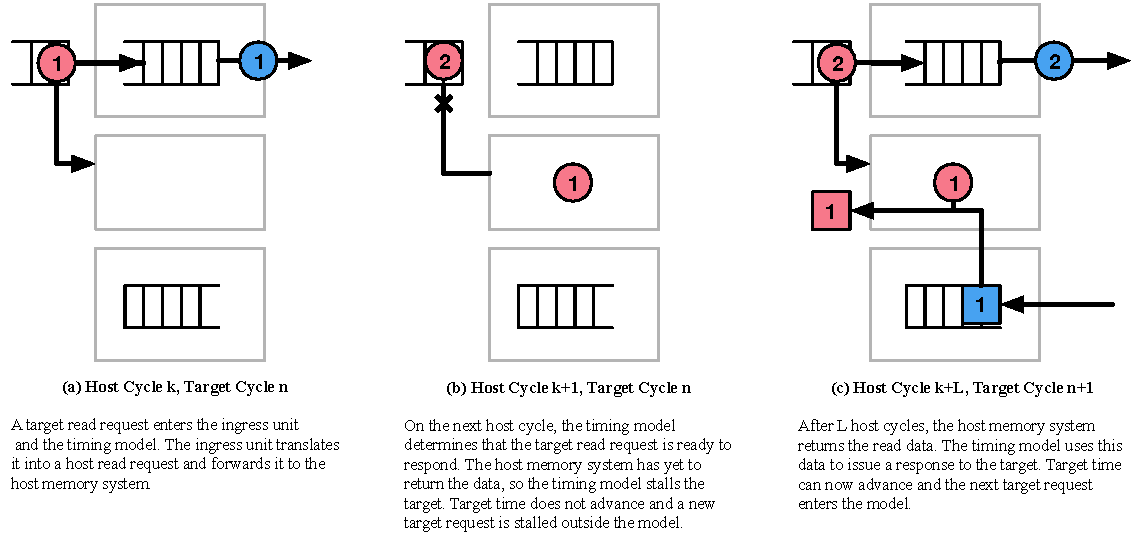
\includegraphics[width=0.8\textwidth]{figures/memory-model-operation.pdf}
\caption{Operation of a single-cycle memory system.}
\label{fig:model_operation} \end{figure}

\section{Generator Configuration}\label{sec:generator-parameters}

There are two points at which the model can be configured.  At
\textit{generation time}, the designer selects an instance. At
\textit{simulation time}, the instance is programmed through via simulation
MMIO through its configuration-side interface. Simulation time configurability
permits the designer to perform parameter sweeps without needing to recompile
the simulator bitstream -- at the expense of FPGA resources. Since both timing
and functional components of an instance are provisioned pessimistically,
giving hints to generator can greatly reduce FPGA resource utilization.

The generator's input configuration consists of a \emph{base} configuration
that is extended with a timing-model configuration .The parameters of the base
configuration are described in the table~\ref{tbl:base-config}. Timing-model
configurations are described section \label{sec:timing-model}.  Note, ingress
and egress unit generation depends only on parameters of the base
configuration.

\begin{table}
\begin{center}
\resizebox{\textwidth}{!}{%
    \begin{tabular}{|p{0.20\textwidth}|p{0.10\textwidth}|p{0.7\textwidth}|}
    \hline
    \textbf{Name} & \textbf{Default} & \textbf{Description} \\
    \hline
    \hline
    \textit{TargetAXIKey} & N/A & Gives the widths of variable width fields in the target-side AXI4 interface. \\
    \hline
    \textit{MaxReads} & N/A & The number of maximum outstanding reads the instance can support.  \\
    \hline
    \textit{MaxWrites} & N/A & As above, for write transactions. \\
    \hline
    \textit{MaxReadLength} & 256 & The maximum number of beats in a read transaction. (Defaults to AXI4 limit.) \\
    \hline
    \textit{MaxWriteLength} & 256 & As above, for write transactions. \\
    \hline
    \textit{MaxReadIDs} & $2^{IDWidth}$ & Specifies a bound on the maximum number of AXI4 read channel IDs that will be used by in-flight requests. \\
    \hline
    \textit{MaxWriteIDs} & $2^{IDWidth}$ & As above, for write transactions. \\
    \hline
\end{tabular}}
\end{center}
\caption{Generator base configuration parameters.}
\label{tbl:base-config}
\end{table}%

\section{Egress Unit Design}\label{sec:egress}

In this section we consider only read responses, as they constitute the bulk of the area of the egress unit.

How the egress unit implements its virtual queues depends on base-generation
parameters (table~\ref{tbl:base-config}), including the maximum number of
requests sharing an ID concurrently,  MaxReadsPerID ($R_{ID,max}$), the maximum
concurrent number of responses across all IDs, MaxReads ($R_{max}$), and the
maximum length, in beats, of a read response, MaxReadLength ($L_{max}$).

The egress unit is provisioned for the worst case, but tries to intelligent
save FPGA resources where possible. To describe the trade off we define virtual
state $VS$ as the total state required to directly implement each virtual
queue:

$$VS = ID_{max}*R{ID,max}*L_{max}*B$$

Where $B$ are the number of bits per beat. We also define ideal state, $IS$,
the state required to store the maximum number of responses of maximum length.

$$IS = R_{max}*L_{max}*B$$

Note that, if the user does not specify a bound on ($R_{ID,max}$, then, all
responses may share a single ID and thus,

$$VS = IS*ID_{max}$$

The conventional wisdom in design for FPGAs is that BRAM is cheap. Instead of
trying to be clever, for small degrees of virtual state, and the egress unit
physical implements each of those queues in BRAM, in a structure called a
SRAMMultiFIFO (SMF)~\cite{smf}. Naturally, this requires $VS$ bits. Since there the egress unit only ever enqueues
into one queue and dequeues from one queue, a 1R-1W port BRAM can be used to
co-locate the entries of multiple queues.  Read and write pointers for each
queue are maintained separately in registers. The AXI IDs and read or write
pointer associated with it's queue are simply concatenated to fetch a beat from
BRAM.

For large virtual state, and when $VS > IS$, directly implementing each virtual
queue in BRAM becomes too expensive. Consider the case in which we assume AXI4
specification maximums of 256 unique IDs and 256 beat transactions, an egress
unit with 64 bit data beats supporting a only 16 responses would have $VS =
8MiB$, but only $IS = 32 KiB$.

Instead, here egress uses a level of indirection, and dynamically assigns
entries in an SMF, with $R_{max}$ queues of depth $L_{max}$, to responses as
they are received. A translation unit contains a free list and a mapping table,
which for each SMF entry has a valid bit, a head bit, an AXI ID and a next
pointer to an entry holding the next oldest response with the same AXI ID. This
establishes a linked list that maintains an age ordering of responses for the
given AXI channel.

When a response from the host is received, it requests an entry in the SMF from
the translation unit. The granted entry is marked valid, and the next youngest
transaction sharing that AXI ID, updates it's next pointer.  The response
proceeds to enqueues into the SMF. When the model requests a response, the
translation unit matches on the head of the linked list of the requested AXI
ID; returning an entry index if there is a hit. The response is then dequeued
from the SMF beat-by-beat as the model handshakes on the egress response port.
Once the final beat has been read from the SMF, the entry is freed, and the
next youngest entry for the AXI ID is marked as the head.

This translation unit is an associative structure that produces an translation
combinationally, and thus tends to be LUT intensive, and may adversely affect
cycle time. To date, our simulations have never been resource constrained, the
critical paths lie in transformed-RTL models, and run with FMR of 1. In the
future, there are many optimizations that could be made to trade time for
area.\footnote{In retrospect, implementing the CAM in BRAM paying an extra
cycle for translation is definitely a better design point.}

Regardless of egress implementation, selecting the right base configuration
parameters can dramatically save resources. Consider the default configuration
of Rocket-Chip, which has an AXI ID width of 4 bits, data width of 64 bits, and
a block size of 64 bytes. Here, a cache refill served in 8 beats -- one eighth
of the AXI4 maximum length -- and can reduce $VS$ from 0.5 MiB to 16
KiB.\footnote{In a Xilinx 7 series architecture, this is 4 36Kb BRAMs ($<$ 1\%
of the BRAM available on the XC7Z045)} Furthermore, in many cases masters do not
issue multiple requests using the same transaction ID to maximize the
flexibility of the slave to reorder requests. Using the same example, and
setting $R_{ID,max}$ to one, sets $VS = IS = 1 KiB$ permitting a direct
implementation to fit in a single BRAM of any modern FPGA architecture.

Presently, the generator uses a direct implementation if $VS <= 32 KiB$ or $VS
= IS$. We leave defining a better heuristic to future work. Ultimately, how
custom-RTL models should be optimized is a system-level question that
depends on the resource utilization the project, desired FMR, and
the host-FPGA architecture. Indeed, simulators under BRAM pressure may wish to use
translation logic when the generator by default may choose otherwise. At time
of writing, MIDAS generated simulators tend to be under LUT pressure. In this
case, even when $VS > IS$, directly implementing the virtual queues may be
desired.

\section{Timing-Model Classes}\label{sec:timing_model}

\subsection{Latency-Bandwidth Pipe}

The latency-bandwidth pipe model applies independently programmable latencies
to read and write requests. It does not accept any new requests beyond a
programmable limit; this serves as a coarse-grain bandwidth bound via Little's
law. Note, for systems that make requests of varying lengths, the simulated
DRAM bandwidth will be reduced when making shorter requests. This model never
reorders target requests.

\noindent Runtime parameters are shown in table~\ref{tbl:lbp-programmable-registers}.

\begin{table}
\begin{center}
\resizebox{\textwidth}{!}{%
    \begin{tabular}{|p{0.20\textwidth}|p{0.8\textwidth}|}
    \hline
    \textbf{Name} & \textbf{Description} \\
    \hline
    \hline
    \textit{ReadMaxRequests} & Sets the maximum number of in-flight write
        requests the timing-model will accept, before apply backpressure to
        request channels. \\
    \hline
    \textit{WriteMaxRequests} & As above, but for write requests. \\
    \hline
    \textit{ReadLatency} & Sets the latency of a read-request. \\
    \hline
    \textit{WriteLatency} & As above, for write transactions. Note, this length
        is measured from the cycle at which both write address and write data
        requests have been completed to the cycle at which the write
        acknowledgment is first produced. \\
    \hline
\end{tabular}}
\end{center}
\caption{Programmable registers of the latency-bandwidth pipe.}
\label{tbl:lbp-programmable-registers}
\end{table}%

\clearpage
\subsection{Bank Conflict}\label{sec:bank-conflict}

The bank conflict model adds a penalty of $max(0, t_{CP} - t_{\Delta})$ to a
base latency if a read or write request used the bank $t_{\Delta}$ cycles
prior, where $t_{CP}$ is the maximum conflict penalty. The model has a
reconfigurable number of banks and bank address assignment.  The bank address
is assigned by setting an offset and a mask, where: $$Address_{Bank} =
(Address_{Physical} >> Offset) \& Mask$$  The timing-model must be provisioned
with the maximum number of banks at generation time. This model may reorder requests.

\noindent Generation and runtime parameters are shown in
tables~\ref{tbl:bc-generator-parameters}
and~\ref{tbl:bc-programmable-registers} respectively.

\begin{table}[htb]
\begin{center}
\resizebox{\textwidth}{!}{%
    \begin{tabular}{|p{0.20\textwidth}|p{0.10\textwidth}|p{0.7\textwidth}|}
    \hline
    \textbf{Name} & \textbf{Default} & \textbf{Description} \\
    \hline
    \hline
    \textit{MaxBanks} & N/A & Specifies the maximum number of banks the timing-model can support. Must be a power of 2. \\
    \hline
    \textit{MaxLatencyBits} & 12 & Defines the number of bits used in cycle accountings of target-time. \\
    \hline
\end{tabular}}
\end{center}
\caption{Additional generation parameters of the bank conflict timing-model.}
\label{tbl:bc-generator-parameters}
\end{table}%

\begin{table}[htb]
\begin{center}
\resizebox{\textwidth}{!}{%
    \begin{tabular}{|p{0.20\textwidth}|p{0.8\textwidth}|}
    \hline
    \textbf{Name} & \textbf{Description} \\
    \hline
    \hline
    \textit{ReadMaxRequests} & Same as latency-bandwidth pipe (table~\ref{tbl:lbp-programmable-registers}) \\
    \hline
    \textit{WriteMaxRequests} & Same as latency-bandwidth pipe (table~\ref{tbl:lbp-programmable-registers}) \\
    \hline
    \textit{Latency} & Sets the base latency of a read or write transaction. \\
    \hline
    \textit{ConflictPenalty} & Sets the maximum number of additional cycles a
        conflicting transaction will be delayed. \\
    \hline
    \textit{BankAddrOffset} & Specifies the position of the LSB of the bank
        address within the physical address.  \\
    \hline
    \textit{BankAddrMask} & Specifies the mask used to extract the bank address from the physical address. \\
    \hline
\end{tabular}}
\end{center}
\caption{Programmable registers of the bank conflict timing-model.}
\label{tbl:bc-programmable-registers}
\end{table}%

\clearpage
\subsection{FCFS DRAM MAS} This class models a FCFS DRAM MAS (see
section~\ref{fcfs}) with programmable open and closed page policies. The FCFS
model has programmable bank and row address assignment which are implemented as
described in section~\ref{sec:bank-conflict}. This model does not reorder
requests.

\noindent Generation and runtime parameters are shown in
tables~\ref{tbl:fcfs-generator-parameters}
and~\ref{tbl:fcfs-programmable-registers}
respectively.

\begin{table}[htb]
\begin{center}
\resizebox{\textwidth}{!}{%
    \begin{tabular}{|p{0.20\textwidth}|p{0.10\textwidth}|p{0.7\textwidth}|}
    \hline
    \textbf{Name} & \textbf{Default} & \textbf{Description} \\
    \hline
    \hline
    \textit{MaxBanks} & N/A & Same as bank-conflict model (table~\ref{tbl:bc-generator-parameters}  \\
    \hline
    \textit{MaxRowAddrBits} & 16 & Specifies the maximum length of a row address. \\
    \hline
\end{tabular}}
\end{center}
\caption{Additional generation parameters of the FCFS DRAM MAS model.}
\label{tbl:fcfs-generator-parameters}
\end{table}%

\begin{table}[htb]
\begin{center}
\resizebox{\textwidth}{!}{%
    \begin{tabular}{|p{0.20\textwidth}|p{0.8\textwidth}|}
    \hline
    \textbf{Name} & \textbf{Description} \\
    \hline
    \textit{tCAS} & Specifies CAS latency. \\
    \hline
    \textit{tRP} & Specifies row precharge delay. \\
    \hline
    \textit{tRCD} & Specifies row-to-column command delay. \\
    \hline
    \textit{ReadMaxRequests} & Same as latency-bandwidth pipe (table~\ref{tbl:lbp-programmable-registers}) \\
    \hline
    \textit{WriteMaxRequests} & Same as latency-bandwidth pipe (table~\ref{tbl:lbp-programmable-registers}) \\
    \hline
    \textit{BankAddrOffset} & Same as bank-conflict model (table~\ref{tbl:bc-programmable-registers}) \\
    \hline
    \textit{BankAddrMask} & Same as bank-conflict model (table~\ref{tbl:bc-programmable-registers}) \\
    \hline
    \textit{RowAddrOffset} & Same mechanism as above for defining row address assignment in physical address. \\
    \hline
    \textit{RowAddrMask} & See above. \\
    \hline
    \textit{OpenPagePolicy} & When set, the model does not close an open row immediately after each request. \\
    \hline
\end{tabular}}
\end{center}
\caption{Programmable registers of the FCFS DRAM MAS model.}
\label{tbl:fcfs-programmable-registers}
\end{table}%

\clearpage
\subsection{FR-FCFS DRAM MAS}
This class models a FR-FCFS (section~\ref{frfcfs}) with an open page policy. It
shares all of the same generation and runtime parameters as the FCFS DRAM MAS
model (tables~\ref{tbl:fcfs-programmable-registers} and \ref{tbl:fcfs-generator-parameters}))


\section{DRAM MAS Model Limitations}

Note that while the latter two models do have programmable $t_{RP}$, $t_{CS}$,
$t_{RCD}$, they are incomplete models of a generic DDR DRAM. We enumerate some
key limitations here:

\begin{enumerate}
    \item\textbf{No refresh model}. Neither model accounts for refresh leading to
        artificially high bandwidths (especially in the FR-FCFS model) and
        depressing tail latency one might see in DRAM typically -- where read
        requests hit a bank currently under refresh.

    \item\textbf{Missing timings}. Models currently do not account for all
        timing DRAM timing constraints. Some notable examples are four row
        activation window ($t_{FAW}$), and row-activation to row-activation
        delay ($t_{RRD}$) which can limit achievable bandwidth when memory
        requests have poor row buffer locality or in MAS that close rows more
        aggressively.

    \item\textbf{No multi-rank support}. Models currently assume single-rank
        memory organizations. Multi-rank organizations have substantial
        implications on MAS policies, as accessing banks in different ranks is
        more expensive then accessing banks on the same rank. In contrast,
        rank-level parallelism in a memory access stream may permit the MAS to
        issue more activation commands than would be legal in a single-rank
        configuration due to $t_{FAW}$ and $t_{RRD}$ constraints.

\end{enumerate}

While software DRAM simulators support multi-channel configurations, in MIDAS
we expect the user will simply use separate model instances for each
controller.  Finally, there is no fundamental limitation of our scheme that
presents us from addressing any of three limitation above. We intend to expand
the fidelity of the DRAM timing-model classes as we use them in the future.



